\documentclass[12pt,a4paper,oneside]{article}
\usepackage[utf8]{vietnam}
\usepackage{amsmath}
\usepackage{amsfonts}
\usepackage{amssymb}
\usepackage{graphicx}
\usepackage[left=2cm,right=2cm,top=2cm,bottom=2cm]{geometry}
\usepackage{array}
\usepackage{fancyhdr}
\pagestyle{fancy}
\renewcommand\thesection{\Roman{section}.}
\renewcommand\thesubsection{\arabic{subsection}.}
\fancyhf{}
\rhead{{\large \textbf{Laboratory Exercise 10.1}}
}
\lhead{Hoàng Quốc Bảo - 20194484}
\rfoot{Trang \thepage}

\usepackage{listings}
\usepackage{tcolorbox}
\usepackage{color} % tô màu cho code
\definecolor{dkgreen}{rgb}{0,0.6,0}
\definecolor{gray}{rgb}{0.5,0.5,0.5}
\definecolor{code}{rgb}{0.8,0.8,0.8}
\definecolor{mauve}{rgb}{0.58,0,0.82}
\lstset{frame=tb,
  language=[x86masm]Assembler,
  aboveskip=3mm,
  belowskip=3mm,
  showstringspaces=false,
  columns=flexible,
  basicstyle={\small\ttfamily},
  backgroundcolor=\color{gray!20!white},
  numbers=none,
  breaklines=true,
  breakatwhitespace=true,
  tabsize=3
}

\begin{document}
\section*{Assignment 1 - LED PORT}
\textbf{Mã nguồn:}
\begin{lstlisting}
.eqv SEVENSEG_LEFT 0xFFFF0011 # Dia chi cua den led 7 doan trai.
 # Bit 0 = doan a; 
 # Bit 1 = doan b; ... 
# Bit 7 = dau .
.eqv SEVENSEG_RIGHT 0xFFFF0010 # Dia chi cua den led 7 doan phai

.text
main:
 li $a0, 0x7f # set value for segments
 jal SHOW_7SEG_LEFT # show
 nop
 li $a0, 0x66 # set value for segments
 jal SHOW_7SEG_RIGHT # show 
 nop
exit: li $v0, 10
 syscall
endmain:
#---------------------------------------------------------------


# Function SHOW_7SEG_LEFT : turn on/off the 7seg
# param[in] $a0 value to shown 
# remark $t0 changed
#---------------------------------------------------------------
SHOW_7SEG_LEFT: li $t0, SEVENSEG_LEFT # assign port's address
 sb $a0, 0($t0) # assign new value 
 nop
jr $ra
nop

#---------------------------------------------------------------


# Function SHOW_7SEG_RIGHT : turn on/off the 7seg
# param[in] $a0 value to shown 
# remark $t0 changed
#---------------------------------------------------------------
SHOW_7SEG_RIGHT: li $t0, SEVENSEG_RIGHT # assign port's address
 sb $a0, 0($t0) # assign new value
 nop
jr $ra 
 nop
\end{lstlisting}
\pagebreak
\textbf{Giải thích:}
\begin{itemize}
\item Hiển thị 2 số cuối MSSV (8 và 4). 
	\begin{itemize}
	\item Muốn hiển thị số 8, chúng ta cho đèn sáng các thanh a-b-c-d-e-f-g. Chuyển sang mã nhị phân 8 bit ta được 0111 1111 = 0x3F.\\Thay vào chương trình:
	\begin{center}
	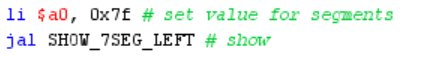
\includegraphics[scale=1]{1}
	\end{center}
	\item Muốn hiển thị số 4, chúng ta cho đèn sáng các thanh b-c-f-g. Chuyển sang mã nhị phân 8 bit ta được 0110 0110 = 0x66.\\Thay vào chương trình:
	\begin{center}
	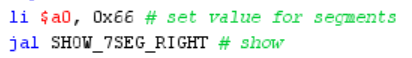
\includegraphics[scale=1]{2}
	\end{center}
	\end{itemize}
\end{itemize}
\textbf{Kết quả thực hiện:}
\begin{center}
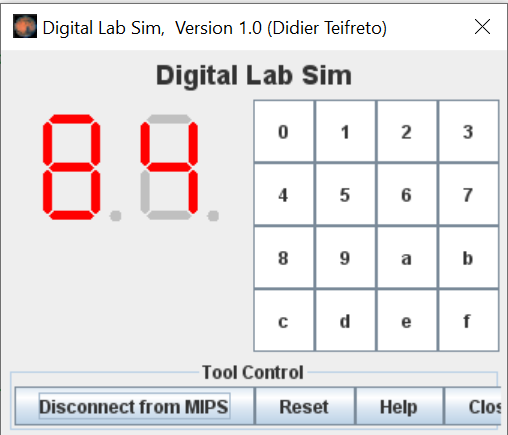
\includegraphics[scale=1]{3}
\end{center}
\pagebreak
\section*{Assignment 2 - BITMAP DISPLAY}
\textbf{Mã nguồn:}
\begin{lstlisting}
.eqv MONITOR_SCREEN 0x10010000 #Dia chi bat dau cua bo nho man hinh
.eqv RED 0x00FF0000 #Cac gia tri mau thuong su dung
.eqv GREEN 0x0000FF00
.eqv BLUE 0x000000FF
.eqv WHITE 0x00FFFFFF
.eqv YELLOW 0x00FFFF00
.text
 li $k0, MONITOR_SCREEN #Nap dia chi bat dau cua man hinh


 li $s1, 0
 li $s2, 252
 li $s3, 4
 li $s4, WHITE
 jal paint		# Background = WHITE
 nop
 
 b1:
 li $s1, 40
 li $s2, 212
 li $s3, 32
 li $s4, RED
 jal paint		
 nop
 
  b2:
 li $s1, 40
 li $s2, 52
 li $s3, 4
 li $s4, RED
 jal paint		
 nop
 
 b3:
 li $s1, 52
 li $s2, 212
 li $s3, 32
 li $s4, RED
 jal paint		
 nop
 
 b4:
 li $s1, 200
 li $s2, 212
 li $s3, 4
 li $s4, RED
 jal paint		
 nop
 
 b5:
 li $s1, 52
 li $s2, 56
 li $s3, 4
 li $s4, WHITE
 jal paint		
 nop
 
  b6:
 li $s1, 212
 li $s2, 214
 li $s3, 4
 li $s4, WHITE
 jal paint		
 nop
 
 b7:
 li $s1, 108
 li $s2, 112
 li $s3, 4
 li $s4, RED
 jal paint		
 nop
 j end
 
 
 paint:
 add $t2, $zero, $s1		# $s1 = begin
 loop:
 bgt $t2, $s2, endloop		# $s2 = end
 nop
 add $t1, $k0, $t2 		# $t1 = address of place
 add $t0, $zero, $s4		# $s4 = COLOR		
 sw $t0, 0($t1)
 add $t2, $t2, $s3		# $s3 = step
 j loop
 nop
 endloop:
 jr $ra
 end:
 \end{lstlisting}
 \textbf{Giải thích:}
 \begin{itemize}
 \item Mục tiêu của chương trình là in ra chữ B.
 \item Chương trình con \textit{paint} thực hiện tô màu cho các vùng địa chỉ được chỉ định (mỗi pixel cách nhau 4 bit địa chỉ)\\Nhận đầu vào là 4 giá trị (địa chỉ tương đối với \$k0):
 	\begin{itemize}
 	\item \$s1: Địa chỉ ô nhớ bắt đầu
 	\item \$s2: Địa chỉ ô nhớ kết thúc
 	\item \$s3: bước nhảy - step (Nếu tô theo hàng ngang thì step = 4, nếu tô theo hàng dọc thì step = 4 * 8 = 32)
 	\item \$s4: Giá trị màu cần tô.
 	\end{itemize}
 	\begin{center}
 	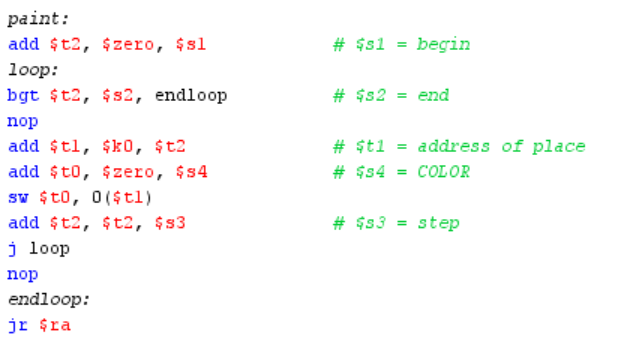
\includegraphics[scale=1]{4}
 	\end{center}
 \item Ban đầu, chúng ta tô màu toàn bộ background bằng nền trắng
 \begin{center}
 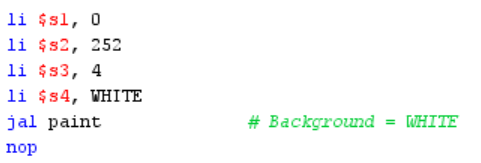
\includegraphics[scale=1]{5}
 \end{center}
 \item Từ các bước \textit{b1} đến \textit{b5}, chúng ta lần lượt dùng hàm \textit{paint} để tô màu ra số 8 trên bảng BITMAP.
 \begin{center}
 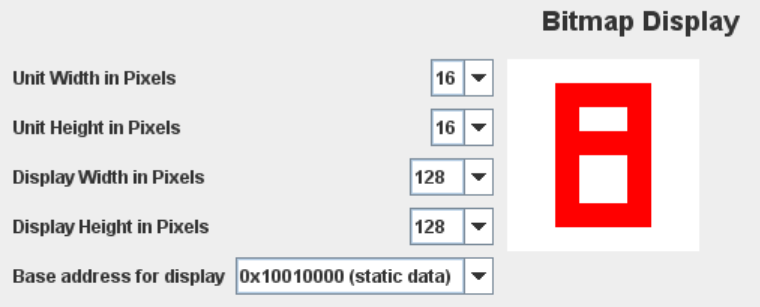
\includegraphics[scale=1]{6}
 \end{center}
 \item Các bước \textit{b6} và \textit{b7}, hoàn thành chữ B bằng cách tô màu trắng 2 góc trên và dưới bên phải.
 \begin{center}
 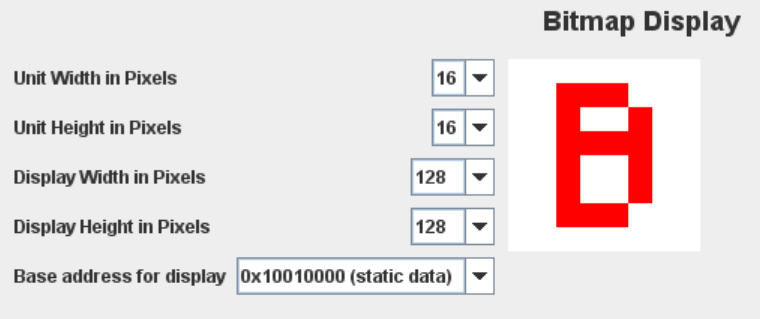
\includegraphics[scale=1]{7}
 \end{center}
 \end{itemize}
 \textbf{Ở mảng Data Segment}:
 \begin{center}
 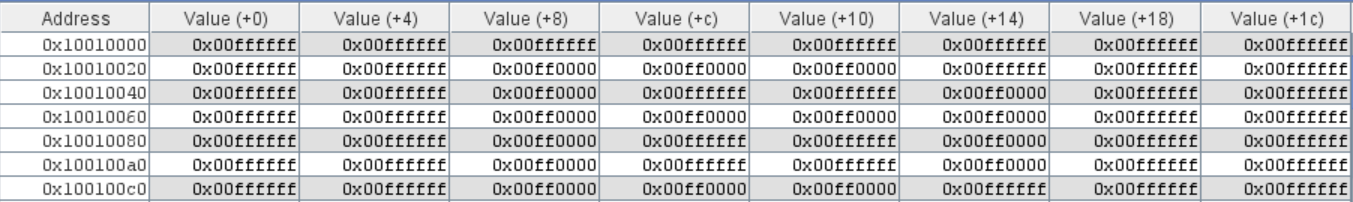
\includegraphics[scale=1]{8}
 \end{center}
 Ta thấy ở địa chỉ đầu tiên 0X10010000 bằng với giá trị thanh ghi \$k0 (MONITOR\_SCREEN). Giá trị 0x00FFFFFF tương ứng với màu trắng. Giá trị 0x00FF0000 tương ứng với giá trị màu đỏ, có vị trí tương ứng với chữ B màu đỏ nền trắng. Mỗi \textit{Value} cách nhau 4 bit tương ứng với mỗi pixel.
\end{document}